\setcounter{page}{1}    % 将页码计数器设置为 1

% ===============================================================
%
% 问题重述与分析
%
% ===============================================================

\section{问题重述}

\subsection{问题背景}

互联网迅猛发展,线上教育平台这种新型教育模式逐渐兴起。各种基于互联网的教育模式渐渐的发展起来了。利用互联网的高度便利性和自定义性,因材施教的程度得到了进一步发展。为了进一步实现用户的个性化学习,某\linebreak MOOC在线教育平台提供了个性化题库的功能。该题库系统会记录用户的学习过程,而自动生成对应的课后习题。但该系统目前来说还存在着很大缺陷。

题目系统为了实现个性化试题,主要是实现两个子功能:\textbf{相似度评估系统}和\textbf{难度评估系统}。

目前而言,这两个系统都有明显的缺陷。

\subsection{相似度评估系统}

该系统中,评判两个题目之间相似度主要依据是\textbf{题干文字}和\textbf{事先标注题目的知识点信息}。前者无法应对不同表述但是解法相同的题目,后者与知识点划分方式相关,难以达到真正的拓展练习的地步,这急需要改进。

\subsection{难度评估系统}

该系统中,判断题目难度的依据主要是\textbf{考试的类型}和\textbf{教师的主观经验}。这两种方式的局限性都太大了,前者只能够判断考试试题的难度,然而还有更多的题目是不会出现在考试试题中的;后者太主观了,不同的老师可能会给出完全不同的两种回答。并且,一个题目难度和题面的表达、学习者的状态、学习者的知识储备等等因素有关。所以,该系统仍然需要进一步改进。

\section{问题分析}

\begin{figure}[h]
    \centering
    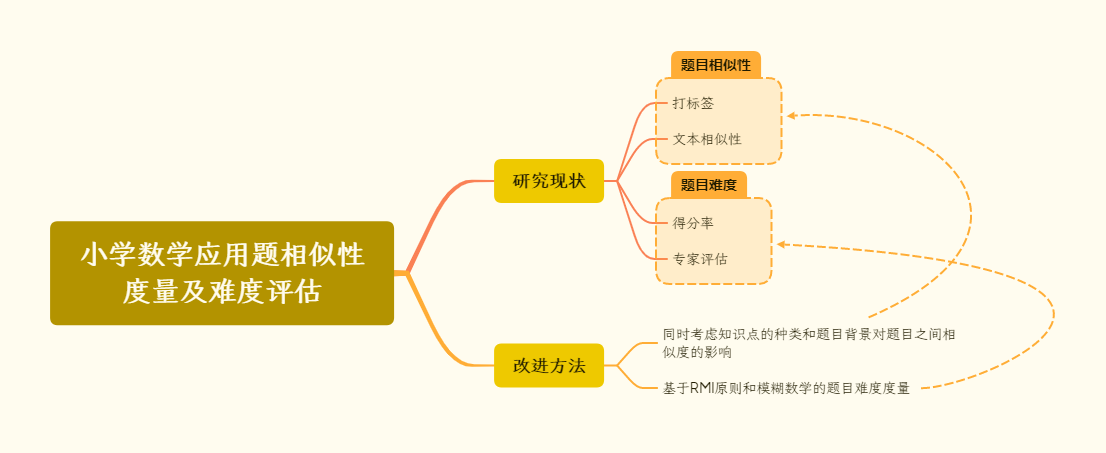
\includegraphics[scale=0.22]{res/figure042227.png}
    \caption{关于相似度和难度评估的改进思路}
\end{figure}
 
\subsection{关于相似度和难度评估的研究现状}

当今学术界对题目相似性的研究主要是局限于文本的相似性,然而,这并不一定是有效的,我们该如何给出对应的感受呢?为了研究这样的内容,可以提高学生的学习效率。从传统上看,关于题目相似性的研究几乎都是从打标签的角度开始的\cite{xuTimunandupinggufangfayanjiuzongshu2022},大概是这样的一个流程。

当今学术界对题目相似性的研究主要是局限于现在“打标签”。打标签是一种多维度分类的方法,通过这样的作法,让题目之间的相似性可以局限在已有的知识体系之中。而对于题目的难度而言,目前研究的主要手段是通过得分率、老师专家的评分。这样没有将题目本身的难度和外在难度区分开来的研究占大部分。

\subsection{同时考虑知识点的种类和题目背景的相似性}

对于两个题目之间的相似性,可以从知识点种类于题目背景两个方面思考。对于题目的知识种类,两个题目所涵盖的知识种类的交集越多,这两个题目之间的相似性显然就越高,同样的,两个题目的应用背景越相似,两个题目的相似性也会越高。对于传统判断题目相似的方法,都只能考虑其中一种可能性,所以,一个更加合理的做法就是同时考虑这两种可能性。

基于以上两点思考,这里通过自然语言处理(Nature Language Processing, NLP)理论中的jieba分析系统和LDA模型处理题目,提取其中的逻辑信息和背景信息。

通过这样的处理,可以较好的改善目前相似性度量系统的缺陷。

\subsection{模糊数学与题目难度评估}

对于题目的难度评估,主要从RMI原则和模糊数学两个方面分析。

\begin{figure}[h]
    \centering
    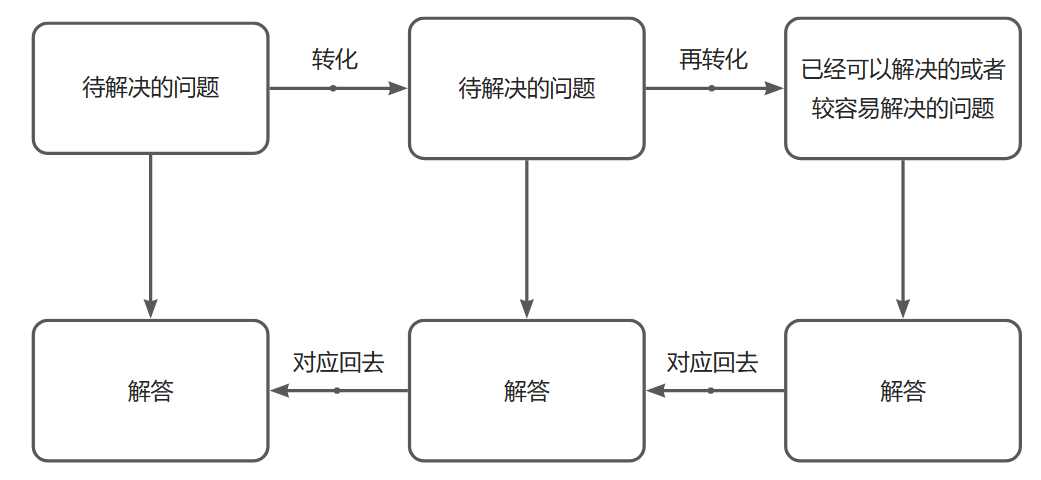
\includegraphics[scale=0.3]{res/figure040117.png}
    \caption{RMI原则}
    \label{figure040117}
\end{figure}

\paragraph{RMI原则}

RMI原则,全称关系-映射-反演(relation-mapping-inversion)原则,是由徐利治先生于上世纪80年代提出的数学方法论\cite{zhangShuxueshitishiqiannandudeyingxiangyinsujiqilianghuayanjiu2022}。该理论认为,解决数学问题的关键在于对于问题“化归”过程,通俗来说,就是将复杂数学问题通过某种认知的方法转化为已经解决的数学问题的过程,也就是化繁为简。基本模式入图\ref{figure040117}所示。

\paragraph{模糊综合评价}

对于一道小学的应用题而言,决定它难度的因素除了其自身的难度而言,还有许多其他因素需要避免。就如前文所言,学习者的状态和知识储备也同样会影响小学应用题的难度。在本文中,对于题目难度的评估都是对题目本身的复杂度的评估,而不考虑其他难度状态。

本文中,主要考虑下面四个因素,其重要性依次递减:

\begin{enumerate}
    \item 知识点数量。一个题目可能包含多个知识点所考察的知识点越多,题目难度越大。
    \item 数学运算的难易。解一元二次方程的难度肯定大于解一元一次方程的难度。
    \item 试题背景的复杂性。对于应用题而言,需要学习者需要将文字数学化,这种数学化的过程难易也会影响应用题本身的难度。
    \item 个人主观评分。有些题目是具有很强技巧性的。虽然它没有考察很多知识点的数量,也没有非常复杂的数学运算和数学背景,但是需要一种巧妙地思考才能解出该题。
\end{enumerate}

\subsection{总思路}

综合以上三个小结的分析,下面给出优化题目相似性度量和题目难度评估方法的总思路(如图\ref{figure042108})。

\begin{figure}[h]
    \centering
    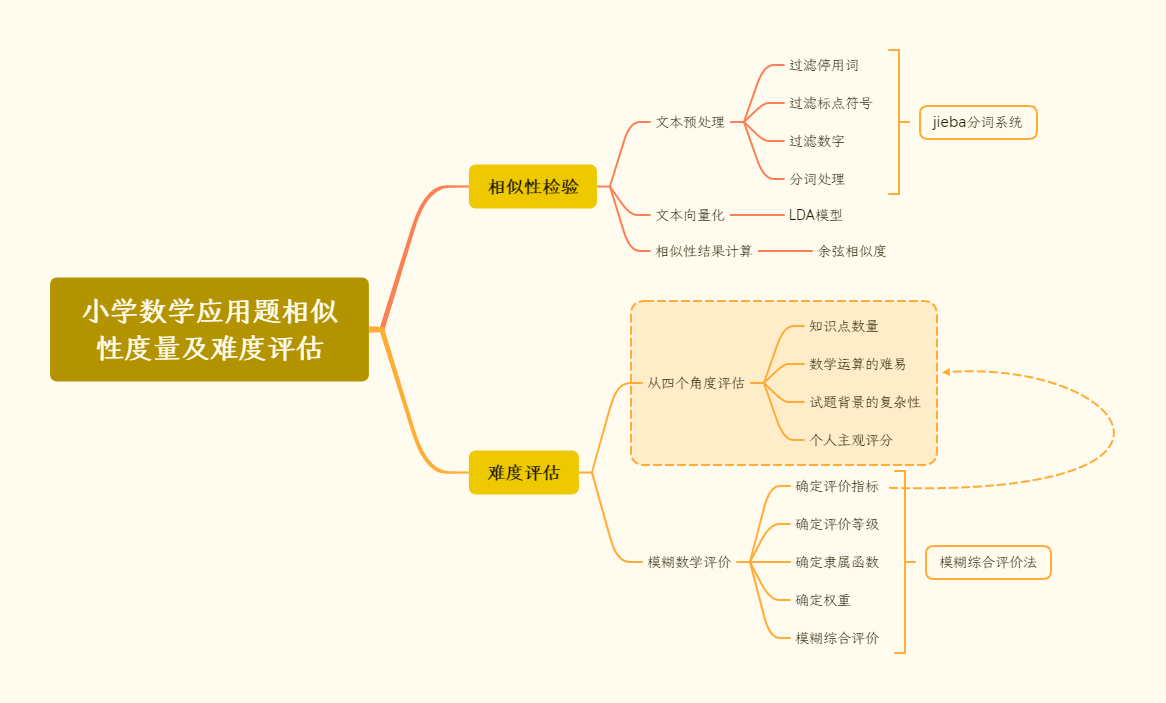
\includegraphics[scale=0.2]{res/figure042108.png}
    \caption{小学数学应用题相似性度量及难度评估的研究的总思路}
    \label{figure042108}
\end{figure}

% ===============================================================
%
% 模型假设与符号说明
%
% ===============================================================

\section{模型假设与符号说明}

\subsection{模型假设}

\begin{itemize}
    \item 假设学习者是小学教育水平;
    \item 假设每个难度评估者都是抱着尽量客观的态度进行评估作业的;
    \item 假设每道应用题都只有唯一种解法;
    \item 假设题库中所考察的知识点是已知且有限的。
\end{itemize}

\subsection{符号说明}

\begin{table}[h]
    \centering
    \begin{tabular}{@{}cc@{}}
        \toprule
        \quad \quad \quad 符号 \quad \quad \quad           & 意义                       \\ \midrule
        $Z_{n,l}$     & 文档$n$中第$l$个分词对应的主题编号     \\
        $\alpha$      & 控制文档-主题分布的超参数/狄利克雷分布先验参数 \\
        $\beta$       & 控制主题-词语分布的超参数/狄利克雷分布先验参数 \\
        $w_{n,l}$     & 文档$n$中第$l$个分词对应的主题编号     \\
        $\varphi_{k}$ & 主题$k$的词汇分布               \\
        $M_{diff}$    & 题目难度矩阵                   \\
        $L_{weight}$  & 题目难度值                    \\
        $L_D$         & 题目难度系数序列                 \\
        $S_{level}$   & 难度度量等级集合                 \\ \bottomrule
    \end{tabular}
\end{table}